\section{Question 1} \label{sec:Q1}

\textbf{\textit{Calculate the sound pressure level in the conference room due to fan noise transmitted through the ductwork (both supply and return).}}


The resolution of the SPL in the conference room due to fan noise, L\textsubscript{p\textsubscript{1}}, is detailed at 63~Hz in Table~\ref{tbl:BN_conf_example} and further explained below.


\subsection{Sound power level leaving a duct}

The first step is to calculate the sound power level leaving a single ductwork, L\textsubscript{W\textsubscript{out}} (see Equation~\ref{eq:power_out}).
In this question, L\textsubscript{W\textsubscript{in}} is the sound power level of the fan.
%These values are provided in Table~1 of the assignment description.
From the fan to the conference room, the fan noise is attenuated five times:
\begin{enumerate}
	\item Within the sound attenuator
	\item Along the 15~m horizontal duct
	\item At the branch
	\item Along the 0.5~m vertical duct
	\item At the duct termination due to end reflection losses
\end{enumerate}
%, is equal to the sound power level that entered the duct, L\textsubscript{W\textsubscript{in}}, minus the sum of all attenuations (assuming all attenuations are positive) (see Equation~\ref{eq:power}).

    \begin{equation}\label{eq:power_out}
		L_{W out} = L_{W in} - \sum Attn
	\end{equation}

%The attenuation provided by the sound attenuator are given in Table~5 of the assignment description.
%The length attenuation of the horizontal and vertical ducts are calculated from values given in Table~4 of the assignment description.
N.B. In the calculation of the attenuation provided by the horizontal duct, we had a choice.
For x\textsubscript{2} = 400~mm, we could either choose an attenuation of 1.00 or 1.64 at 63~Hz.
Since we have decided to calculate for a worst case scenario, we chose the lower range of attenuation values (i.e. for a side dimension between 200~mm and 400~mm).
So the attenuation at 63~Hz, Attn\textsubscript{x\textsubscript{2}63}, is 1.00.


\subsection{SPL in the conference room from a single ductwork}

The second step is to calculate the SPL in the conference room from a single ductwork.
Equation~\ref{eq:SPL} shows how to calculate the SPL in a room.

	\begin{equation}\label{eq:SPL}
		L_{p} = L_{W} - 10 log \frac{V}{T} + 14
	\end{equation}


\subsection{Sum SPLs from both ducts}

The final step is to sum the SPLs from both the supply and return ducts.
Since both ducts have the same sound power level entering and the same attenuations, the SPLs are the same.
For this calculation, we use the rule of thumb for summing two identical SPLs by adding three decibels, i.e. L\textsubscript{p\textsubscript{double}} = L\textsubscript{p\textsubscript{single}} + 3.


\subsection{L\textsubscript{p\textsubscript{1}} results at all frequencies}

The L\textsubscript{p\textsubscript{1}} results are presented in octave bands between 63~Hz and 4~kHz in Table~\ref{tbl:BN_conf}.

It is interesting to note that the SPLs at 63~Hz and 125~Hz are low relative to the other SPLs.
This is largely because of the high end reflection losses at low frequencies.
%The wavelengths are too long to come through the 'grille'; they get bounced back into the vertical duct.

\textbf{Add details of hrzl to vertical branch attenuation calculation}

\begin{sidewaystable}[htbp]
	\caption{Details of the calculation of the SPL in the conference room due to fan noise, L\textsubscript{p\textsubscript{1}}, at 63~Hz.}
	\label{tbl:BN_conf_example}
	\centering
	\begin{tabular}{@{}m{5cm}rm{10cm}@{}}
		\toprule
		Frequency (Hz) & 63 & Notes \\ \midrule
		L\textsubscript{W\textsubscript{fan}} (dB re 10\textsuperscript{-12} W) & 92 & Given in Table~1 of assignment description \\
		&  &  \\
		Attn\textsubscript{sound attenuator} (dB) & 6 & Given in Table~5 of assignment description \\
		&  &  \\
		Attn\textsubscript{horizontal} (dB) & $15 \times (1.64 + 1) = 39.6$ & \begin{tabular}[c]{@{}l@{}}According to Table~4 of assignment description:\\ For x\textsubscript{1} = 600~mm, the attenuation at 63~Hz, Attn\textsubscript{x\textsubscript{1}63}, is 1.64.\\ For x\textsubscript{2} = 400~mm, the attenuation at 63~Hz, Attn\textsubscript{x\textsubscript{2}63}, is 1.00.\\ Length attenuation = duct length $\times$ (Attn\textsubscript{x\textsubscript{1}63} + Attn\textsubscript{x\textsubscript{2}63}).\end{tabular} \\
		&  &  \\
		Attn\textsubscript{horizontal $\rightarrow$ vertical} (dB) & $\left|10 log \frac{0.12}{0.12 + 0.24}\right| = 4.77$ & $\left|10 log \frac{S_{vertical}}{S_{vertical} + S_{horizontal}}\right|$ \\
		&  &  \\
		Attn\textsubscript{vertical} (dB) & $0.5 \times (1 + 1) = 1.00$ & Same as notes for Attn\textsubscript{horizontal}, but for x\textsubscript{1} = 300~mm and x\textsubscript{2}~=~400~mm \\
		&  &  \\
		Attn\textsubscript{end reflections} (dB) & 11 & Given in Table~6 of assignment description for a duct cross-sectional area of 0.3~m $\times$ 0.4~m = 0.12~m\textsuperscript{2} \\
		&  &  \\
		$\Sigma$Attn (dB) & 62.37 & Sum of all attenuations \\
		&  &  \\
		L\textsubscript{W\textsubscript{out}} (dB re 10\textsuperscript{-12} W) & $92 - 62.37 = 29.63$ & $L_{W out} = L_{W fan} - \Sigma Attn$ \\
		&  &  \\
		T\textsubscript{1} (s) & 0.48 & From Table~\ref{tbl:reverb_conf} \\
		&  &  \\
		SPL in conference room due to single ductwork, L\textsubscript{p\textsubscript{1 single}} (dB) & $29.63 - 10 log \frac{80}{0.48} + 14 = 21.45$ & \begin{tabular}[c]{@{}l@{}} $L_{p_1 single} = L_{W out} – 10 log \frac{V_1}{T_{1_{63}}} + 14$\end{tabular} \\
		&  &  \\
		SPL in conference room due to supply and return, L\textsubscript{p\textsubscript{1}} (dB) & $21.45 + 3 = 24.4$ & Sum of two identical SPLs = $L_p + 3$ \\ \bottomrule
	\end{tabular}
\end{sidewaystable}

% Please add the following required packages to your document preamble:
% \usepackage{booktabs}
\begin{table}[htbp]
	\caption{Calculation of the SPL in the conference room due to fan noise, L\textsubscript{p\textsubscript{1}}.}
	\label{tbl:BN_conf}
	\centering
	\begin{tabular}{@{}m{8cm}rrrrrrr@{}}
		\toprule
		Frequency (Hz) & 63 & 125 & 250 & 500 & 1000 & 2000 & 4000 \\ \midrule
		L\textsubscript{W\textsubscript{fan}} (dB re 10\textsuperscript{-12} W) & 92 & 94 & 94 & 93 & 92 & 88 & 84 \\
		Attn\textsubscript{sound attenuator} (dB) & 6 & 9 & 16 & 27 & 31 & 30 & 21 \\
		Attn\textsubscript{horizontal} (dB) & 39.6 & 39.6 & 24.9 & 14.7 & 5.85 & 5.85 & 5.85 \\
		Attn\textsubscript{horizontal $\rightarrow$ vertical} (dB) & 4.77 & 4.77 & 4.77 & 4.77 & 4.77 & 4.77 & 4.77 \\
		Attn\textsubscript{vertical} (dB) & 1.00 & 1.32 & 1.00 & 0.66 & 0.23 & 0.23 & 0.23 \\
		Attn\textsubscript{end reflections} (dB) & 11 & 7 & 3 & 1 & 0 & 0 & 0 \\
		$\Sigma$Attn (dB) & 62.37 & 61.69 & 49.67 & 48.13 & 41.85 & 40.85 & 31.85 \\
		L\textsubscript{W\textsubscript{out}} (dB re 10\textsuperscript{-12} W) & 29.63 & 32.31 & 44.33 & 44.87 & 50.15 & 47.15 & 52.15 \\
		T\textsubscript{1} (s) & 0.48 & 0.44 & 0.47 & 0.49 & 0.37 & 0.32 & 0.30 \\
		SPL in conference room due to single ductwork, L\textsubscript{p\textsubscript{1 single}} (dB) & 21.4 & 23.7 & 36.0 & 36.7 & 40.8 & 37.1 & 41.9 \\
		SPL in conference room due to supply and return, L\textsubscript{p\textsubscript{1}} (dB) & 24.4 & 26.7 & 39.0 & 39.7 & 43.8 & 40.1 & 44.9 \\ \bottomrule
	\end{tabular}
\end{table}

\begin{figure}[htbp]
	\centering
	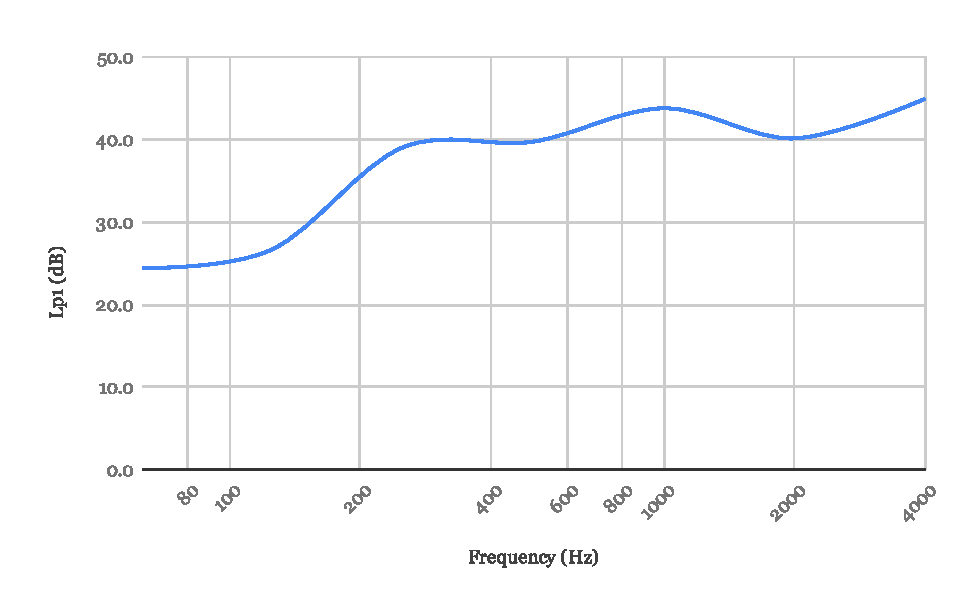
\includegraphics[width=\textwidth]{figures/Lp1.eps}
	\rule{\textwidth}{0.5pt} % use line???
	\caption{The SPL in the conference room due to fan noise transmitted through the ductwork (both supply and return), L\textsubscript{p\textsubscript{1}}.}
	\label{fig:Lp1}
\end{figure}